\documentclass[a4paper,12pt]{book}
\usepackage[margin=0.7in,nomarginpar]{geometry}
\usepackage[utf8]{inputenc}
\usepackage{graphicx}
\usepackage{mathtools}
\usepackage{amsfonts}
\usepackage{hyperref}
\usepackage{tabularx}
\usepackage{array}
\usepackage[table]{xcolor}
\usepackage{circuitikz}
\usepackage{polynom}
\usepackage{pstricks}
\usepackage{wrapfig}
\usepackage[italian]{babel}
\usepackage{float}
\restylefloat{table}
\usepackage{mathtools}
\usepackage{fancyvrb}
\usepackage{listings}
\graphicspath{ {./images/} }

\DeclarePairedDelimiter\ceil{\lceil}{\rceil}
\DeclarePairedDelimiter\floor{\lfloor}{\rfloor}

\addtolength{\topmargin}{.2in}
\addtolength{\textheight}{-.3in}

\newcommand{\overbar}[1]{\mkern 1.5mu\overline{\mkern-1.5mu#1\mkern-1.5mu}\mkern 1.5mu}

\newcommand{\diagram}[2]{
	\begin{figure}[H]
	\centering
	\input{./diagrams/#1}
	\caption{#2}
	\end{figure}
}

\def\C{\mathbb{C}}
\def\N{\mathbb{N}}
\def\Q{\mathbb{Q}}
\def\R{\mathbb{R}}
\def\Z{\mathbb{Z}}

% Code Listings
\definecolor{vgreen}{RGB}{104,180,104}
\definecolor{vblue}{RGB}{49,49,255}
\definecolor{vorange}{RGB}{255,143,102}
\lstset{
	basicstyle=\ttfamily,
	columns=fullflexible,
	keepspaces=true,
}
\lstdefinestyle{verilog} {
	language=Verilog,
	basicstyle=\ttfamily,
	keywordstyle=\color{vblue},
	identifierstyle=\color{black},
	commentstyle=\color{vgreen},
	numbers=left,
	numberstyle=\color{black},
	numbersep=10pt,
	tabsize=8,
	moredelim=*[s][\colorIndex]{[}{]},
	literate=*{:}{:}1
}
\lstdefinestyle{bash} {
	language=bash,
	basicstyle=\ttfamily,
	keywordstyle=\color{vblue},
	identifierstyle=\color{black},
	commentstyle=\color{vgreen},
	tabsize=4,
	moredelim=*[s][\colorIndex]{[}{]},
	literate=*{:}{:}1
}

\newcommand{\includecode}[3][c]{\lstinputlisting[caption=#3, style=#1]{#2}}


\begin{document}

\author{Alessandro Cheli - Prof. Marco Danelutto}
\title{Appunti di Architettura degli Elaboratori}
\date{A.A 2019-2020}

\frontmatter
\maketitle
\tableofcontents

\mainmatter
\part{}
\chapter{Introduzione al Corso}

\begin{itemize}
	\item{\textbf{Logica Booleana}}
	\item{\textbf{Aritmetica Binaria}}
	\item{\textbf{Reti Logiche}}
	\item{\textbf{Microarchitettura e Assembler ARM v7 e v8}}
	\item{\textbf{Gestione della memoria}}
	\item{\textbf{I/O}}
\end{itemize}


\begin{defn}
	\textbf{Strumenti Software} \\

	A differenza degli A.A passati utilizzeremo Verilog e Assembler ARM.
	Utilizzeremo \textbf{iverilog} come compilatore Verilog e \textbf{gtkwave} come tool grafico. Un ambiente di sviluppo Verilog completo che vedremo è \textbf{Quartus}.
	Per la seconda parte del corso, Assembler ARM, useremo la \textbf{toolchain GNU}, in particolare:
	
	
	\subparagraph{Se non hai una macchina ARM:}
	\begin{itemize}
		\item{cross-compiler per compilare}
		\item{QEMU per una macchina virtuale ARM}
		\item{gdb per debugging}
	\end{itemize}
	
	\subparagraph{Se hai una macchina ARM come un Raspberry Pi:}
	\begin{itemize}
		\item{Toolchain GNU per compilare}
		\item{Cavo Ethernet}
		\item{Server SSH sulla macchina ARM per accesso remoto}
	\end{itemize}
\end{defn}

\begin{note}
	\textbf{Storia degli Elaboratori}\\
	
	\begin{figure}
		\centering
		\caption{Sinclair ZX80}
		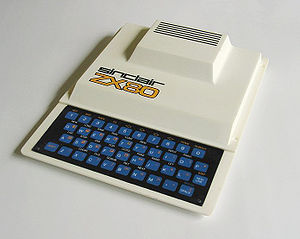
\includegraphics[width=0.5\textwidth]{ZX80}
	\end{figure}
	
	Nei corsi di Architettura degli Elaboratori negli anni 80 i processori studiati erano: il 6502 (8 bit, processore del computer Apple II, noto per essere stato costruito nel garage di Steve Jobs e Wozniak), Z80, processore a 16 bit del famoso computer ZX80 e l'Intel 8088. Tali processori raggiungevano al massimo una velocità di clock (detto molto a grandi linee, operazioni al secondo) dell'ordine di meno di una decina di MHz (Mega Hertz, milioni). I processori odierni raggiungono
	cicli di clock sull'ordine dei GHz (Giga Hertz, miliardi). Nel corso degli anni fino ad oggi, l'evoluzione dei processori ha seguito la \textbf{legge di Moore}. La "legge" spiega che ogni 18 mesi la potenza dei processori in commercio raddoppia, perché la densità dei transistor contenuti all'interno aumenta. Negli ultimi decenni abbiamo  miglioramenti architetturali come super pipeline e super scalari, ciò ha permesso di introdurre processori \textbf{multicore}, ovvero che contengono più "nuclei" interni (detti core) che elaborano le istruzioni dei processi in esecuzione in parallelo.
	Ad oggi il numero di core in uno smartphone raggiunge anche gli 8 core, mentre in processori per server sono stati raggiunti numeri di core anche intorno ai 64. I processori odierni utilizzano core a 64 bit, con architettura X86\_64 per Desktop o ARM per dispositivi mobili.
	Un componente fondamentale dell'evoluzione degli elaboratori è stato anche lo sviluppo dei processori grafici (GPU) con i quali ad oggi è possibile riprodurre grafica su schermo, ambienti tridimensionali molto complessi (videogiochi) o sfruttare la loro capacità di parallelizzazione per l'uso di reti neurali nell'intelligenza artificiale.
	
	Osserveremo i calcolatori a diversi livelli di \textbf{astrazione}
	
	I livelli di astrazione sono:
	\begin{itemize}
		\item Applicazioni utente
		\item Sistema Operativo
		\item Architettura (ASM, ad es. x86 o ARM)
		\item Microarchitettura
		\item Logica
		\item Circuiti digitali
		\item Device
		\item Fisica
	\end{itemize}
	
	Ogni livello si appoggia sul livello inferiore, ovvero è costruito sui componenti offerti dal livello inferiore. Dei principi fondamentali sono: \textbf{gerarchi, modularità e regolarità}
	
	La modularità è fondamentale per avere moduli organizzati gerarchicamente, autonomi ed indipendenti.
\end{note}



\begin{defn}
	\textbf{Set di Istruzioni}

	Distinguiamo due set di istruzioni dei processori, \textbf{CISC} e \textbf{RISC}. Gli acronimi sono rispettivamente \textbf{Complex Instruction Set Computer} e \textbf{Reduced Instruction Set Computer}, RISC contiene i processori ARM, che studieremo in dettaglio, mentre CISC comprende i processori più comuni nei desktop (X86 e X86\_64)
\end{defn}


\chapter{Rappresentazioni Numeriche e Testuali}

\section{Aritmetica Binaria}

I calcolatori utilizzano valori discreti (differenze di potenziale) fra 0 e 1 per rappresentare valori numerici. Viene detta Aritmetica Binaria l'aritmetica con i numeri rappresentati in base 2.

Siamo abituati a ragionare in base 10, ad esempio il numero 413 in base 10 è 
\[ 104 = 10^2 \cdot 1 + 10^1 \cdot 0 + 10^0 \cdot 4 \]

Lo stesso numero rappresentato in base 2 (codice binario) è

\[ 104_{10} = 01101000_2 = 2^7 \cdot 0 + 2^6 \cdot 1 + 2^5 \cdot 1 + 2^4 \cdot 0 + 2^3 \cdot 1 + 2^2 \cdot 0 + 2^1 \cdot 0 + 2^0 \cdot 0 \]

Un numero binario di 8 cifre è detto \textbf{byte}, un numero di 4 cifre è detto \textbf{nibble}. Una \textbf{parola} (\textbf{word}) è la quantità minima su cui viene rappresentato un intero in un calcolatore. Ad oggi le parole dei calcolatori sono 64 bit, alcuni calcolatori datati hanno parole da 32 bit.

La somma nell'aritmetica binaria è definita normalmente per i numeri positivi. Nei calcolatori i numeri hanno una dimensione finita (numero di bit) che indica il numero di cifre binarie con le quali è possibile rappresentare un numero. I positivi binari rappresentano numeri fino a $ 2^{N}-1 $ dove $ N $ è il numero di cifre.

Per rappresentare i numeri negativi si utilizza il metodo \textbf{segno-magnitudo} dove il bit più a sinistra rappresenta il segno (0 se il numero è positivo e 1 se è negativo). Il problema del metodo segno-magnitudo è che non rispetta la somma aritmetica. Può rappresentare numeri da $ [-2^{N-1}, +2^{N-1} ] $

Un metodo migliore per rappresentare i numeri negativi è il \textbf{complemento a due}. Nel complemento a due la cifra più a sinistra rappresenta sempre $ 2^{N-1} $ ma \textbf{negativo}. Il resto delle cifre sono positive e vengono sommate alla prima cifra negativa. Questo metodo rispetta la somma aritmetica. Per moltiplicare un numero per $ -1 $ si invertono le cifre binarie e si aggiunge 1 al numero. È possibile anche la sottrazione sommando un numero positivo ad uno negativo.

La somma fra due cifre può essere costruita con reti logiche. Il risultato della somma $ A + B = A \oplus B $ (operatore XOR) mentre il riporto della somma = $ A \land B $ (operatore AND)

\begin{figure}
	\centering
	\caption{Gate XOR}
	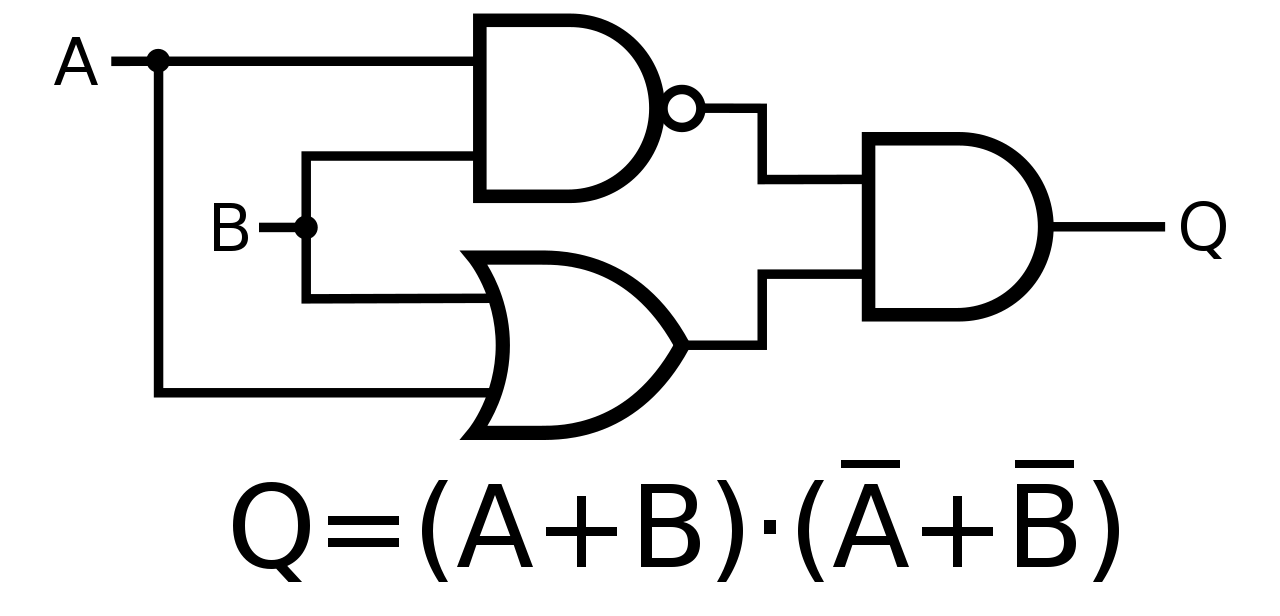
\includegraphics[width=\textwidth/2]{xor}
\end{figure}

\section{Esadecimale} 

I numeri esadecimali sono numeri in base 16. Siccome non bastano le cifre decimali per rappresentare i numeri maggiori di 9 si usano le prime lettere dell'alfabeto.
Una cifra esadecimale rappresenta un nibble (4 bit).

\section{Numeri in virgola mobile}

I numeri in virgola mobile si rappresentano con lo standard EEE 754 che definisce come si rappresentano i numeri in virgola mobile a singola precisione e doppia precisione (32 e 64 bit)

I bit del numero vengono divisi in 3 parti. Il primo bit denota il segno, la seconda parte rappresenta l'esponente e la terza parte si denota mantissa. L'esponente esprime dove la virgola verrà posizionata, come nella notazione scientifica di una calcolatrice l'esponente rappresenta $ 10^{n} $ dove $ n $ è l'esponente. La mantissa è un numero di base moltiplicato per $ 10^0 $, e viene successivamente moltiplicato per l'esponente.
L'esponente può essere sia positivo che negativo.

\begin{figure}
	\caption{Standard IEEE 754 a 32 bit}
	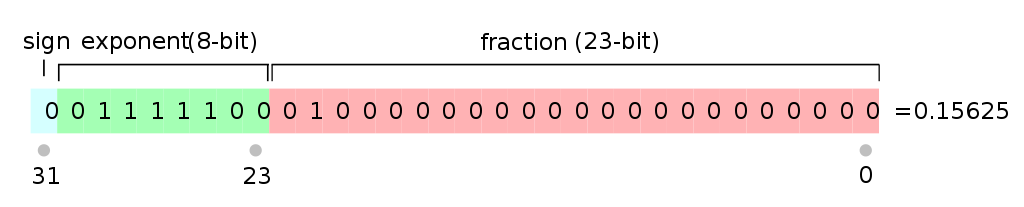
\includegraphics[width=\textwidth]{eee_floating_32}
\end{figure}

Nello standard a 32 bit la sezione esponente ha 8 bit di lunghezza. Un numero ad 8 bit può rappresentare numeri da 0 a 255, per ottenere gli esponenti negativi nello standard dei numeri a virgola mobile il numero a 8 bit rappresenta invece numeri da -127 a +128

\begin{figure}
	\caption{IEEE 754 a 64 bit}
	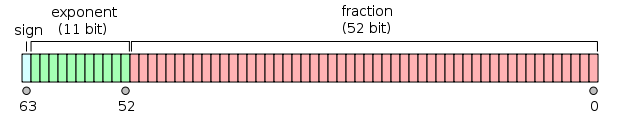
\includegraphics[width=\textwidth]{eee_floating_64}
\end{figure}

\paragraph{Somma dei numeri a virgola mobile}

Per sommare i numeri a virgola mobile il primo passo è allineare le mantisse, significa osservare gli esponenti e spostarli fino a che le cifre non sono sommabili in colonna.
Il secondo passo consiste nel sommare e il terzo passo nel normalizzare la somma. Nei processori la somma floating point viene eseguita in dei moduli appositi che in input ricevono due o più numeri floating point ed eseguono in dei sotto-moduli i tre passaggi della somma in un tempo $ 1/3 t $ dove $ t $ è il tempo totale per eseguire una somma. I tre passaggi della somma possono essere sequenzializzati così che una volta che ogni sotto-modulo ha completato il passo, può ricevere subito l'input successivo (la somma di due numeri FP impiegherà $ t + 1/3 $ invece che $ 2t $)

\paragraph{Estensioni vettoriali}
Alcuni processori permettono di eseguire operazioni contemporaneamente su un registro dividendolo in sottoregistri più piccoli. 

\section{Codifica ASCII}
La codifica ASCII è una tabella di codifica di caratteri testuali con interi da 0 a 255 (8 bit). La codifica ASCII estesa è a 16 bit e comprende diversi caratteri non latini.

\begin{figure}
	\caption{Tabella ASCII}
	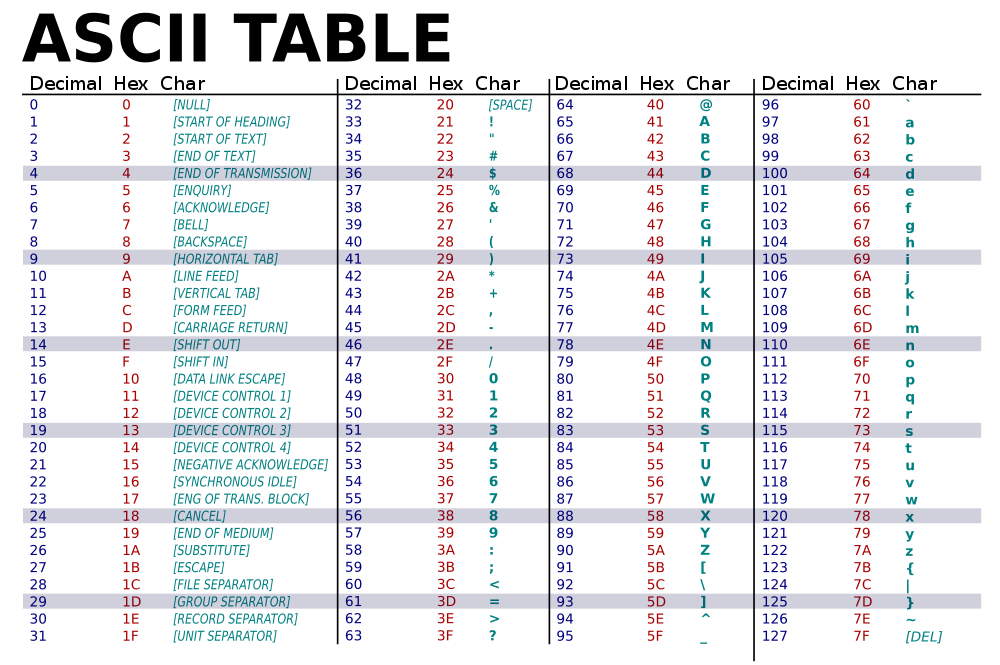
\includegraphics[width=\textwidth]{ascii}
\end{figure}

\section{Porte Logiche e Algebra di Boole}

I circuiti digitali vengono realizzati utilizzando componenti chiamati \textbf{porte logiche}. Sono realizzate con componenti fisici come transistor e resistenze, ma nella progettazione dei circuiti digitali le porte logiche vengono schematizzate con i simboli riportati nella Figura 3.1 per semplificare la progettazione \textbf{astraendo} il livello di complessità della circuiteria analogica.
Solamente con la porta NAND si possono realizzare tutte le altre porte (NAND è funzionalmente completo), ma le porte in generale si costruiscono singolarmente con componenti appositi. Esse implementano la \textbf{logica booleana} che conseguentemente permette di realizzare operazioni di \textbf{aritmetica binaria} per costruire unità di calcolo in componenti elettronici e processori.

\begin{wrapfigure}{r}{0.6\textwidth}
	\begin{center}
		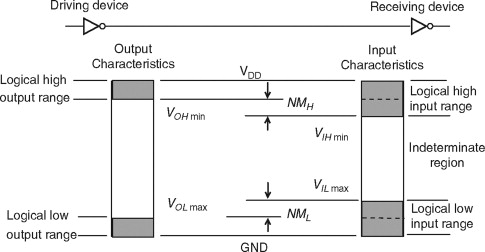
\includegraphics[width=0.58\textwidth]{noisemargin}
	\end{center}
	\caption{Margine di rumore nei circuiti digitali}	
\end{wrapfigure}


I componenti elettronici molto piccoli sono sensibili al \textbf{rumore}, per ovviare al problema i valori discreti (0 e 1) nei circuiti digitali non seguono un cambiamento istantaneo di differenza di potenziale (voltaggio), ma ammettono un margine per ridurre i problemi causati dal rumore.


I componenti (transistor) con cui si costruiscono porte logiche e circuiti sono realizzati con materiali semiconduttori, che possono essere di diversi tipi. Vedremo il tipo NMOS. Un transistor è composto da materiali come gallio e silicio.

\begin{wrapfigure}{r}{0.7\textwidth}
	\begin{center}
		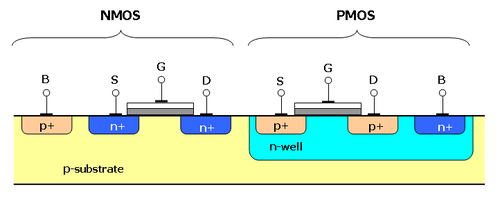
\includegraphics[width=0.68\textwidth]{cmos}
	\end{center}
	\caption{Transistor NMOS}
\end{wrapfigure}


\begin{figure}
	\centering
	\caption{Tabella delle porte logiche comuni}
	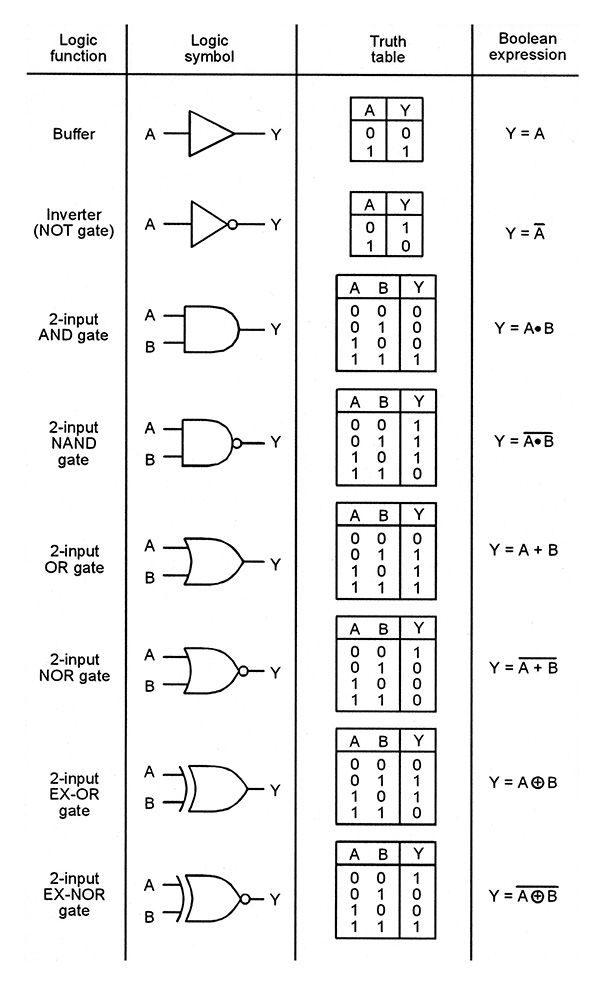
\includegraphics[width=\textwidth,height=\textheight]{logicgates}
\end{figure}

\begin{figure}
	\centering
	\caption{Porta NOT con transistor PMOS e NMOS}
	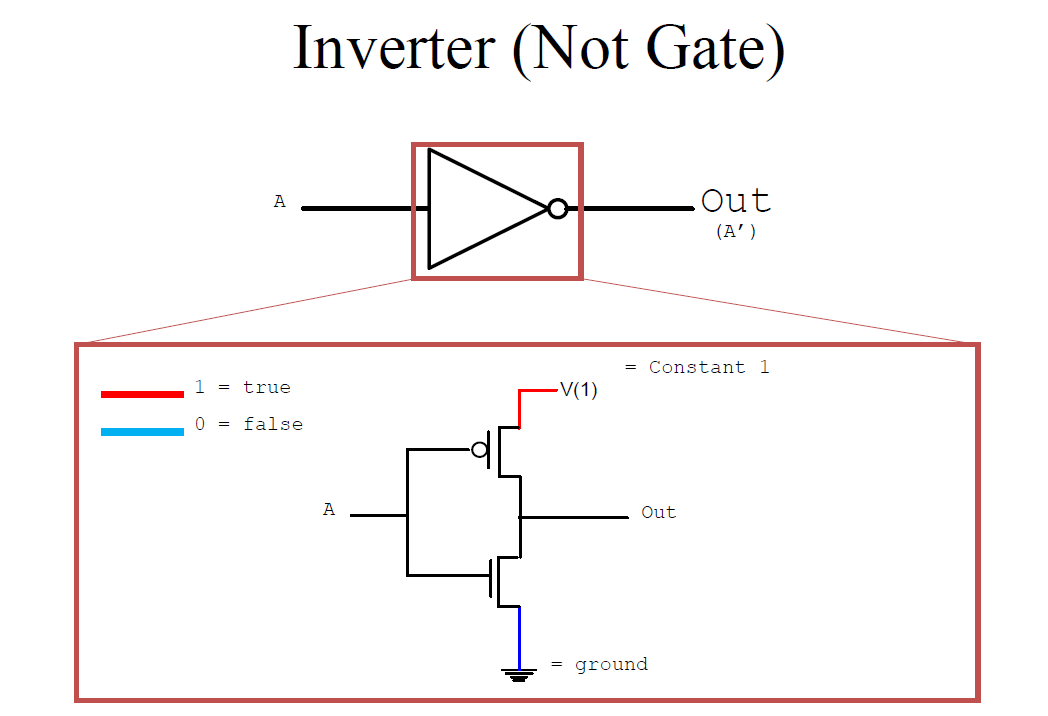
\includegraphics[width=\textwidth]{notgatetransistor}
\end{figure}

\begin{figure}
	\centering
	\caption{Transistor NMOS e PMOS}
	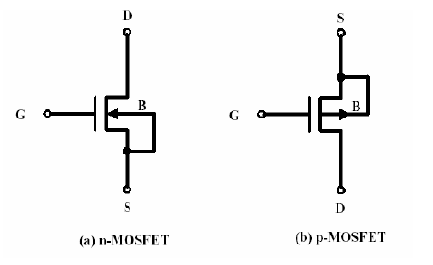
\includegraphics[width=0.6\textwidth]{NMOS-and-PMOS}
\end{figure}

\clearpage

\subsection{Algebra di Boole}


\begin{figure}[H]
	\centering
	
\includegraphics[width=0.48\textwidth]{sommadiprodotti-gate}
	\caption{Conversione di $ z $ da formula booleana a circuito logico}
\end{figure}

\begin{table}[H]
	\centering
	\caption{Notazione usata per l'Algebra di Boole}
	\label{tab:notazione-booleana}
	\begin{tabular}{|l|l|l|}
		\hline
		Funzione & Notazione Usata & Notazione Logica \\ 
		NOT(A)   & $\overbar{A}$   & $\lnot A$        \\ 
		AND(A,B) & $A \cdot B$     & $A \land B$      \\ 
		OR(A,B)  & $A + B$         & $A \lor B$       \\ \hline
	\end{tabular}
\end{table}

Prendiamo ad esempio un espressione booleana in forma canonica in \textbf{somma di prodotti}:
\[ z = \overbar{A}\overbar{B}\overbar{C} + \overbar{A}\overbar{B}C + \overbar{A}BC + A\overbar{B}C + ABC \]


\begin{table}[H]
	\centering
	\caption{Tabella di verità di $ z $}
	\label{tab:z-truth}
	\begin{tabular}{|l|l|l|l|}
		\hline
		A & B & C & z \\ \hline
		0                       & 0                      & 0 & 1 \\  
		0                       & 0                      & 1 & 1 \\ 
		0                       & 1                      & 0 & 0 \\ 
		0                       & 1                      & 1 & 1 \\ 
		1                       & 0                      & 0 & 0 \\ 
		1                       & 0                      & 1 & 1 \\  
		1                       & 1                      & 0 & 0 \\ 
		1                       & 1                      & 1 & 1 \\ \hline
	\end{tabular}
\end{table}




$ z $ si può anche esprimere come prodotto di somme: $ z = (A+\overbar{B}+C)(\overbar{A}BC)(\overbar{A}\overbar{B}C) $


\subsection{Teoremi dell'Algebra Booleana}
Breve ripasso dei teoremi della Logica Booleana.
\paragraph{Elemento Identità di prodotto e somma}
\[ A \cdot 1 = A \iff A \land T \equiv A\]
\[ A + 0 = 0 \iff A \lor F \equiv A\]
\paragraph{Elemento assorbente}
\[ A \cdot 0 = 0 \iff A \land F \equiv F \]
\[ A + 1 = 1 \iff A \lor T \equiv T \]
\paragraph{Idempotenza}
\[ A \cdot A = A \iff A \land A \equiv A \]
\[ A + A = A \iff A \lor A \equiv A \]
\paragraph{Complemento}
\[ A \cdot \overbar{A} = 0 \iff A \land \lnot A \equiv F \]
\[ A + \overbar{A} = 1 \iff A \lor \lnot A \equiv T \]
\paragraph{Commutatività}
\[ A + B = B + A \]
\[ A \cdot B = B \cdot A \]
\paragraph{Associatività}
\[ (A \cdot B) \cdot C = A \cdot (B \cdot C) \]
\[ (A + B) + C = A + (B + C) \]
\paragraph{Distributività}
\[ (A \cdot B) + C = (A+C) \cdot (B+C) \]
\[ (A+B) \cdot C = AC + BC \]
\paragraph{DeMorgan}
\[ \overbar{(A + B)} = \overbar{A} \cdot \overbar{B} \iff \lnot(A \lor B )\equiv \lnot A \land \lnot B \]
\[ \overbar{(A \cdot B)} = \overbar{A} + \overbar{B} \iff \lnot(A \land B )\equiv \lnot A \lor \lnot B \]

\paragraph{Esempio}
Semplifichiamo la formula booleana $ z = \overbar{A}\overbar{B}\overbar{C} + \overbar{A}\overbar{B}C + \overbar{A}BC + A\overbar{B}C + ABC $

\begin{align}
\begin{cases}
\overbar{A}\overbar{B}\overbar{C} + \overbar{A}\overbar{B}C \equiv \overbar{A}\overbar{B}(\overbar{C}+C) \equiv \overbar{A}\overbar{B} \\ 
A\overbar{B}C + ABC \equiv AC(\overbar{B}+B) \equiv AC
\end{cases} \\
\implies z = \overbar{A}\overbar{B} + \overbar{A}BC + AC
\end{align}

Le leggi della logica Booleana ci permettono di semplificare molto i componenti realizzati con porte logiche.

\subsection{Mappe di Karnaugh}

Una mappa di Karnaugh o K-Map è un metodo di semplificare un espressione booleana. I valori sono trasferiti da una tabella di verità ad una mappa bidimensionale:

Approfondisci su \href{https://en.wikipedia.org/wiki/Karnaugh_map}{Wikipedia}

Prendiamo una formula a quattro variabili $ f(A,B,C,D) $, una mappa di Karnaugh può essere:
\begin{table}[H]
	\centering
	\caption{Tabella di verità della mappa di Karnaugh di $f$}
	\label{tab:karnaugh}
	\begin{tabular}{lllll}
		AB\textbackslash{}CD    & 00                     & 01                     & 11                     & 10                     \\ \cline{2-5} 
		\multicolumn{1}{l|}{00} & \multicolumn{1}{l|}{1} & \multicolumn{1}{l|}{1} & \multicolumn{1}{l|}{1} & \multicolumn{1}{l|}{1} \\ \cline{2-5} 
		\multicolumn{1}{l|}{01} & \multicolumn{1}{l|}{1} & \multicolumn{1}{l|}{1} & \multicolumn{1}{l|}{0} & \multicolumn{1}{l|}{0} \\ \cline{2-5} 
		\multicolumn{1}{l|}{11} & \multicolumn{1}{l|}{0} & \multicolumn{1}{l|}{1} & \multicolumn{1}{l|}{0} & \multicolumn{1}{l|}{0} \\ \cline{2-5} 
		\multicolumn{1}{l|}{10} & \multicolumn{1}{l|}{0} & \multicolumn{1}{l|}{0} & \multicolumn{1}{l|}{1} & \multicolumn{1}{l|}{1} \\ \cline{2-5} 
	\end{tabular}
\end{table}

Facciamo ad esempio la mappa di Karnaugh di $ z = f(A,B,C) $ vista nella sezione precedente:

\begin{table}[H]
	\centering
	\caption{Tabella di verità della mappa di Karnaugh di $z$}
	\label{tab:karnaugh}
	\begin{tabular}{lllll}
		A\textbackslash{}BC    & 00                     & 01                     & 11                     & 10                     \\ \cline{2-5} 
		\multicolumn{1}{l|}{0} & \multicolumn{1}{l|}{1} & \multicolumn{1}{l|}{1} & \multicolumn{1}{l|}{1} & \multicolumn{1}{l|}{0} \\ \cline{2-5} 
		\multicolumn{1}{l|}{1} & \multicolumn{1}{l|}{0} & \multicolumn{1}{l|}{1} & \multicolumn{1}{l|}{1} & \multicolumn{1}{l|}{0} \\ \cline{2-5} 
	\end{tabular}
\end{table}

Possiamo riconoscere un'implicante nella seconda e terza colonna che corrisponde esattamente a C. Osserviamo un'altra implicante nella prima riga, prima e seconda colonna che corrisponde esattamente a $ \overbar{A}\overbar{B} $. Possiamo poi sommare le implicanti per ottenere una formula equivalente a quella di partenza, ciò implica che $ z =  \overbar{A}\overbar{B} + C $


\subsection{Circuito con più output}
Se abbiamo una tabella di verità di un circuito con $ n $ input e $ 2^n $ righe, con più output $ z_1, \dots, z_k $, gli output si suddividono in $ k $ tabelle con un solo output ($ z_k $) e $ 2^n $ righe di input.

\subsection{Operatori a più ingressi}
Gli operatori a più ingressi AND, OR, etc..., se presentano più di due ingressi si rappresentano con una rete logica che sfrutta la proprietà associativa degli operatori logici. Ciò comporta un limite massimo di ingressi perché viene introdotto un ritardo di stabilizzazione determinato e piccolo.
Ad esempio, un AND a 4 ingressi sarà rappresentato come $ z = x_1 \cdot x_2 \cdot x_3 \cdot x_4 = (x_1 \cdot x_2 ) \cdot (x_3 \cdot x_4)  $
Perciò gli operatori associativi a più ingressi si rappresentano come un albero k-ario di porte logiche. Il numero di livelli di porte sarà $ log_k(n) $ dove $ k $ è l'arietà delle singole porte ed è $ n $ il numero di ingressi nel circuito.

% TODO figura albero di AND con 8 input. 


\chapter{Porte Logiche e Algebra di Boole}

I circuiti digitali vengono realizzati utilizzando componenti chiamati \textbf{porte logiche}. Sono realizzate con componenti fisici come transistor e resistenze, ma nella progettazione dei circuiti digitali le porte logiche vengono schematizzate con i simboli riportati nella Figura 3.1 per semplificare la progettazione \textbf{astraendo} il livello di complessità della circuiteria analogica.
Solamente con la porta NAND si possono realizzare tutte le altre porte (NAND è funzionalmente completo), ma le porte in generale si costruiscono singolarmente con componenti appositi. Esse implementano la \textbf{logica booleana} che conseguentemente permette di realizzare operazioni di \textbf{aritmetica binaria} per costruire unità di calcolo in componenti elettronici e processori.

\begin{wrapfigure}{r}{0.6\textwidth}
	\begin{center}
		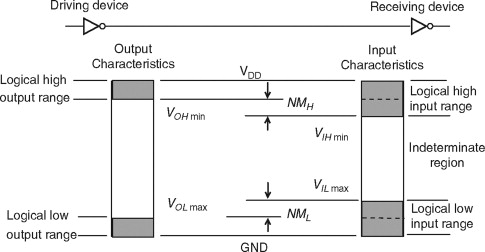
\includegraphics[width=0.58\textwidth]{noisemargin}
	\end{center}
	\caption{Margine di rumore nei circuiti digitali}	
\end{wrapfigure}


I componenti elettronici molto piccoli sono sensibili al \textbf{rumore}, per ovviare al problema i valori discreti (0 e 1) nei circuiti digitali non seguono un cambiamento istantaneo di differenza di potenziale (voltaggio), ma ammettono un margine per ridurre i problemi causati dal rumore.


I componenti (transistor) con cui si costruiscono porte logiche e circuiti sono realizzati con materiali semiconduttori, che possono essere di diversi tipi. Vedremo il tipo NMOS. Un transistor è composto da materiali come gallio e silicio.

\begin{wrapfigure}{r}{0.7\textwidth}
	\begin{center}
		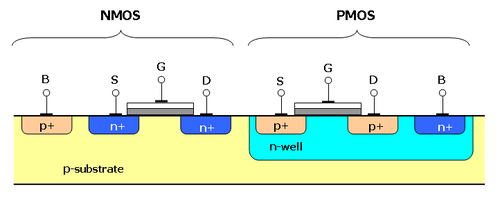
\includegraphics[width=0.68\textwidth]{cmos}
	\end{center}
	\caption{Transistor NMOS}
\end{wrapfigure}


\begin{figure}
	\centering
	\caption{Tabella delle porte logiche comuni}
	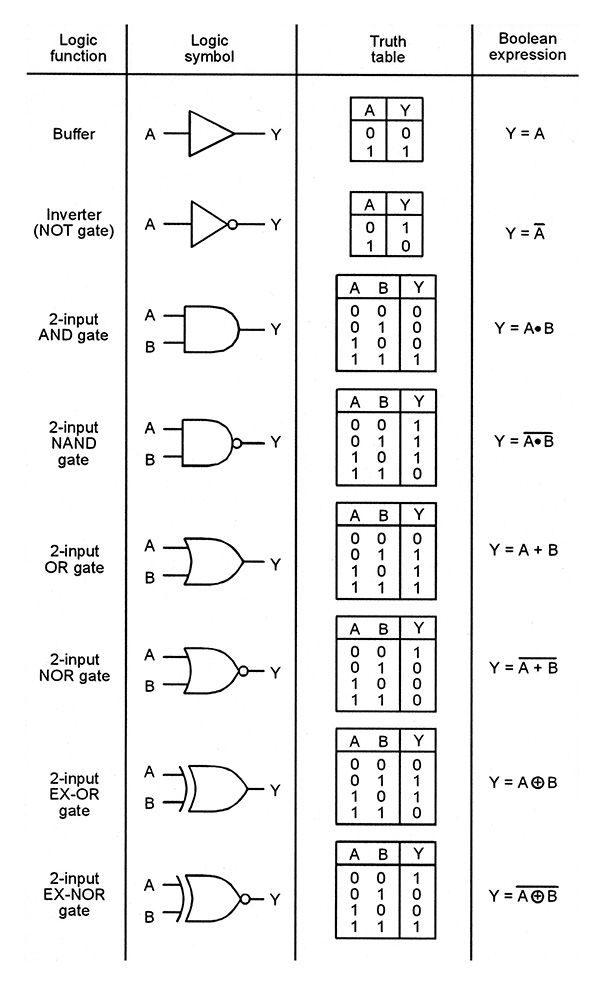
\includegraphics[width=\textwidth,height=\textheight]{logicgates}
\end{figure}

\begin{figure}
	\centering
	\caption{Porta NOT con transistor PMOS e NMOS}
	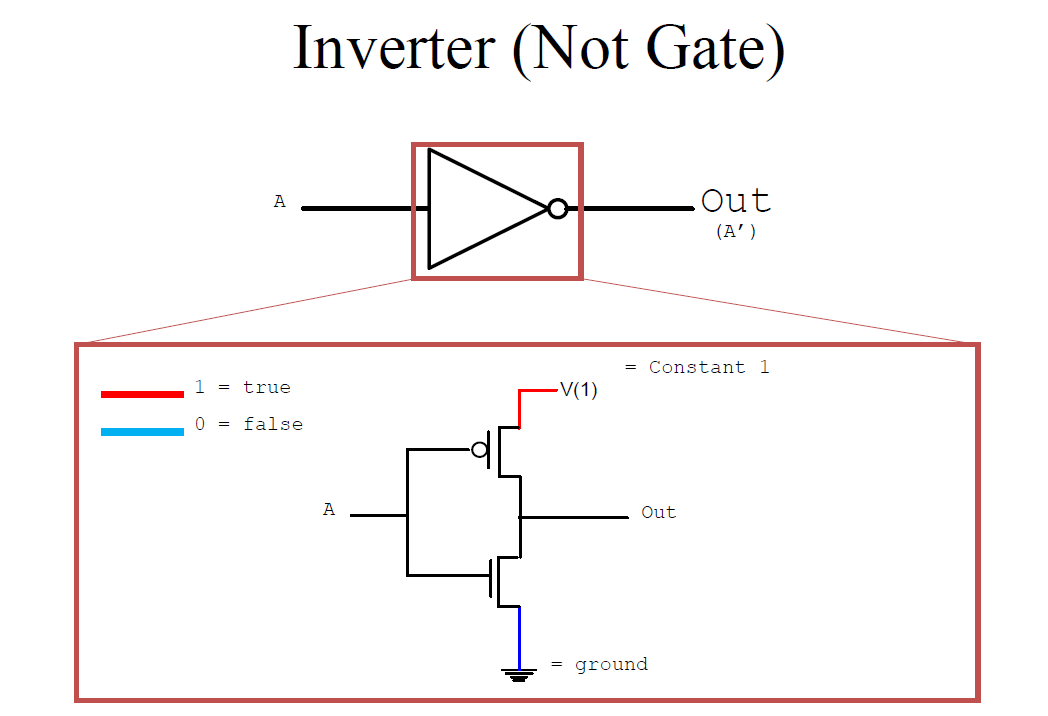
\includegraphics[width=\textwidth]{notgatetransistor}
\end{figure}

\begin{figure}
	\centering
	\caption{Transistor NMOS e PMOS}
	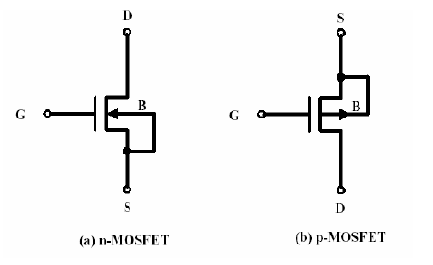
\includegraphics[width=0.6\textwidth]{NMOS-and-PMOS}
\end{figure}

\clearpage

% TODO porta logica NOT con MOS


\section{Algebra di Boole}

\begin{table}[H]
	\centering
	\caption{Notazione usata per l'Algebra di Boole}
	\label{tab:notazione-booleana}
	\begin{tabular}{|l|l|l|}
		\hline
		Funzione & Notazione Usata & Notazione Logica \\ 
		NOT(A)   & $\overbar{A}$   & $\lnot A$        \\ 
		AND(A,B) & $A \cdot B$     & $A \land B$      \\ 
		OR(A,B)  & $A + B$         & $A \lor B$       \\ \hline
	\end{tabular}
\end{table}

La forma canonica di espressioni booleane in \textbf{somma di prodotti} è:
\[ z = \overbar{A}\overbar{B}\overbar{C} + \overbar{A}\overbar{B}C + \overbar{A}BC + A\overbar{B}C + ABC \]

\begin{table}[H]
	\centering
	\caption{Tabella di verità di $ z $}
	\label{tab:z-truth}
	\begin{tabular}{|l|l|l|l|}
		\hline
		A & B & C & z \\ \hline
		0                       & 0                      & 0 & 1 \\  
		0                       & 0                      & 1 & 1 \\ 
		0                       & 1                      & 0 & 0 \\ 
		0                       & 1                      & 1 & 1 \\ 
		1                       & 0                      & 0 & 0 \\ 
		1                       & 0                      & 1 & 1 \\  
		1                       & 1                      & 0 & 0 \\ 
		1                       & 1                      & 1 & 1 \\ \hline
	\end{tabular}
\end{table}

$ z $ si può anche esprimere come prodotto di somme: $ z = (A+\overbar{B}+C)(\overbar{A}BC)(\overbar{A}\overbar{B}C) $

% TODO conversione da forma canonica somma di prodotti a circuito 4.3

\section{Teoremi dell'Algebra Booleana}
Breve ripasso dei teoremi della Logica Booleana.
\paragraph{Elemento Identità di prodotto e somma}
\[ A \cdot 1 = A \iff A \land T \equiv A\]
\[ A + 0 = 0 \iff A \lor F \equiv A\]
\paragraph{Elemento assorbente}
\[ A \cdot 0 = 0 \iff A \land F \equiv F \]
\[ A + 1 = 1 \iff A \lor T \equiv T \]
\paragraph{Idempotenza}
\[ A \cdot A = A \iff A \land A \equiv A \]
\[ A + A = A \iff A \lor A \equiv A \]
\paragraph{Complemento}
\[ A \cdot \overbar{A} = 0 \iff A \land \lnot A \equiv F \]
\[ A + \overbar{A} = 1 \iff A \lor \lnot A \equiv T \]
\paragraph{Commutatività}
\[ A + B = B + A \]
\[ A \cdot B = B \cdot A \]
\paragraph{Associatività}
\[ (A \cdot B) \cdot C = A \cdot (B \cdot C) \]
\[ (A + B) + C = A + (B + C) \]
\paragraph{Distributività}
\[ (A \cdot B) + C = (A+C) \cdot (B+C) \]
\[ (A+B) \cdot C = AC + BC \]
\paragraph{DeMorgan}
\[ \overbar{(A + B)} = \overbar{A} \cdot \overbar{B} \iff \lnot(A \lor B )\equiv \lnot A \land \lnot B \]
\[ \overbar{(A \cdot B)} = \overbar{A} + \overbar{B} \iff \lnot(A \land B )\equiv \lnot A \lor \lnot B \]

\paragraph{Esempio}
Semplifichiamo la formula booleana $ z = \overbar{A}\overbar{B}\overbar{C} + \overbar{A}\overbar{B}C + \overbar{A}BC + A\overbar{B}C + ABC $

\begin{align}
\begin{cases}
\overbar{A}\overbar{B}\overbar{C} + \overbar{A}\overbar{B}C \equiv \overbar{A}\overbar{B}(\overbar{C}+C) \equiv \overbar{A}\overbar{B} \\ 
A\overbar{B}C + ABC \equiv AC(\overbar{B}+B) \equiv AC
\end{cases} \\
\implies z = \overbar{A}\overbar{B} + \overbar{A}BC + AC
\end{align}

Le leggi della logica Booleana ci permettono di semplificare molto i componenti realizzati con porte logiche.

\section{Mappe di Karnaugh}

% TODO cos'è una mappa di Karnaugh

Prendiamo una formula a quattro variabili $ f(A,B,C,D) $, una mappa di Karnaugh può essere:
\begin{table}[H]
	\centering
	\caption{Tabella di verità della mappa di Karnaugh di $f$}
	\label{tab:karnaugh}
	\begin{tabular}{lllll}
		AB\textbackslash{}CD    & 00                     & 01                     & 11                     & 10                     \\ \cline{2-5} 
		\multicolumn{1}{l|}{00} & \multicolumn{1}{l|}{1} & \multicolumn{1}{l|}{1} & \multicolumn{1}{l|}{1} & \multicolumn{1}{l|}{1} \\ \cline{2-5} 
		\multicolumn{1}{l|}{01} & \multicolumn{1}{l|}{1} & \multicolumn{1}{l|}{1} & \multicolumn{1}{l|}{0} & \multicolumn{1}{l|}{0} \\ \cline{2-5} 
		\multicolumn{1}{l|}{11} & \multicolumn{1}{l|}{0} & \multicolumn{1}{l|}{1} & \multicolumn{1}{l|}{0} & \multicolumn{1}{l|}{0} \\ \cline{2-5} 
		\multicolumn{1}{l|}{10} & \multicolumn{1}{l|}{0} & \multicolumn{1}{l|}{0} & \multicolumn{1}{l|}{1} & \multicolumn{1}{l|}{1} \\ \cline{2-5} 
	\end{tabular}
\end{table}

Facciamo ad esempio la mappa di Karnaugh di $ z = f(A,B,C) $ vista nella sezione precedente:

\begin{table}[H]
	\centering
	\caption{Tabella di verità della mappa di Karnaugh di $z$}
	\label{tab:karnaugh}
	\begin{tabular}{lllll}
		A\textbackslash{}BC    & 00                     & 01                     & 11                     & 10                     \\ \cline{2-5} 
		\multicolumn{1}{l|}{0} & \multicolumn{1}{l|}{1} & \multicolumn{1}{l|}{1} & \multicolumn{1}{l|}{1} & \multicolumn{1}{l|}{0} \\ \cline{2-5} 
		\multicolumn{1}{l|}{1} & \multicolumn{1}{l|}{0} & \multicolumn{1}{l|}{1} & \multicolumn{1}{l|}{1} & \multicolumn{1}{l|}{0} \\ \cline{2-5} 
	\end{tabular}
\end{table}

Possiamo riconoscere un'implicante nella seconda e terza colonna che corrisponde esattamente a C. Osserviamo un'altra implicante nella prima riga, prima e seconda colonna che corrisponde esattamente a $ \overbar{A}\overbar{B} $. Possiamo poi sommare le implicanti per ottenere una formula equivalente a quella di partenza, ciò implica che $ z =  \overbar{A}\overbar{B} + C $


\subsection{Circuito con più output}
Se abbiamo una tabella di verità di un circuito con $ n $ input e $ 2^n $ righe, con più output $ z_1, \dots, z_k $
\chapter{Reti Sequenziali, Verilog e RTL}

Gli RTL, o Register Transfer Language, permettono di descrivere cosa succede a livello di circuito fra registri. Vengono utilizzati per descrivere l'hardware. Vedremo il linguaggio \textbf{Verilog}. Gli RTL permettono di descrivere e comporre dei moduli. Il libro di testo propone il dialetto \textbf{System Verilog} che mette a disposizione due metodi per descrivere i moduli. Un metodo è il metodo \textit{constructive}, noi vedremo il metodo \textit{behavioral} dove ad esempio un Multiplexer da 2 vie 1 bit è descritto da:
\begin{lstlisting}[style={verilog}]
	z = (ic == 0 ? x : y)
\end{lstlisting}

Verilog è un linguaggio compilato. Un file System Verilog compilato produce una traccia di esecuzione e un eseguibile che simula il comportamento dei moduli. Viene detta \textbf{simulazione}.

Un programma Verilog può anche essere dato in input a un programma detto \textbf{synthetizer}, che produce una \textbf{netlist}, ovvero una lista dei componenti e dei collegamenti per realizzare il modulo fisicamente. Un altro modo per realizzare la sintesi è utilizzare un \textbf{FPGA}, o Field-programmable gate array. Un FPGA è un circuito integrato composto da una matrice di celle, e una singola cella può:
\begin{enumerate}
	\item Eseguire una funzione booleana di 3-5 ingressi con 1 uscita 
	\item Implementare un bit di memoria
	\item Routing
\end{enumerate} 

Un FPGA moderno comprende, oltre a delle celle, delle righe che contengono diversi componenti come delle ALU.

\begin{figure}[H]
	\centering
	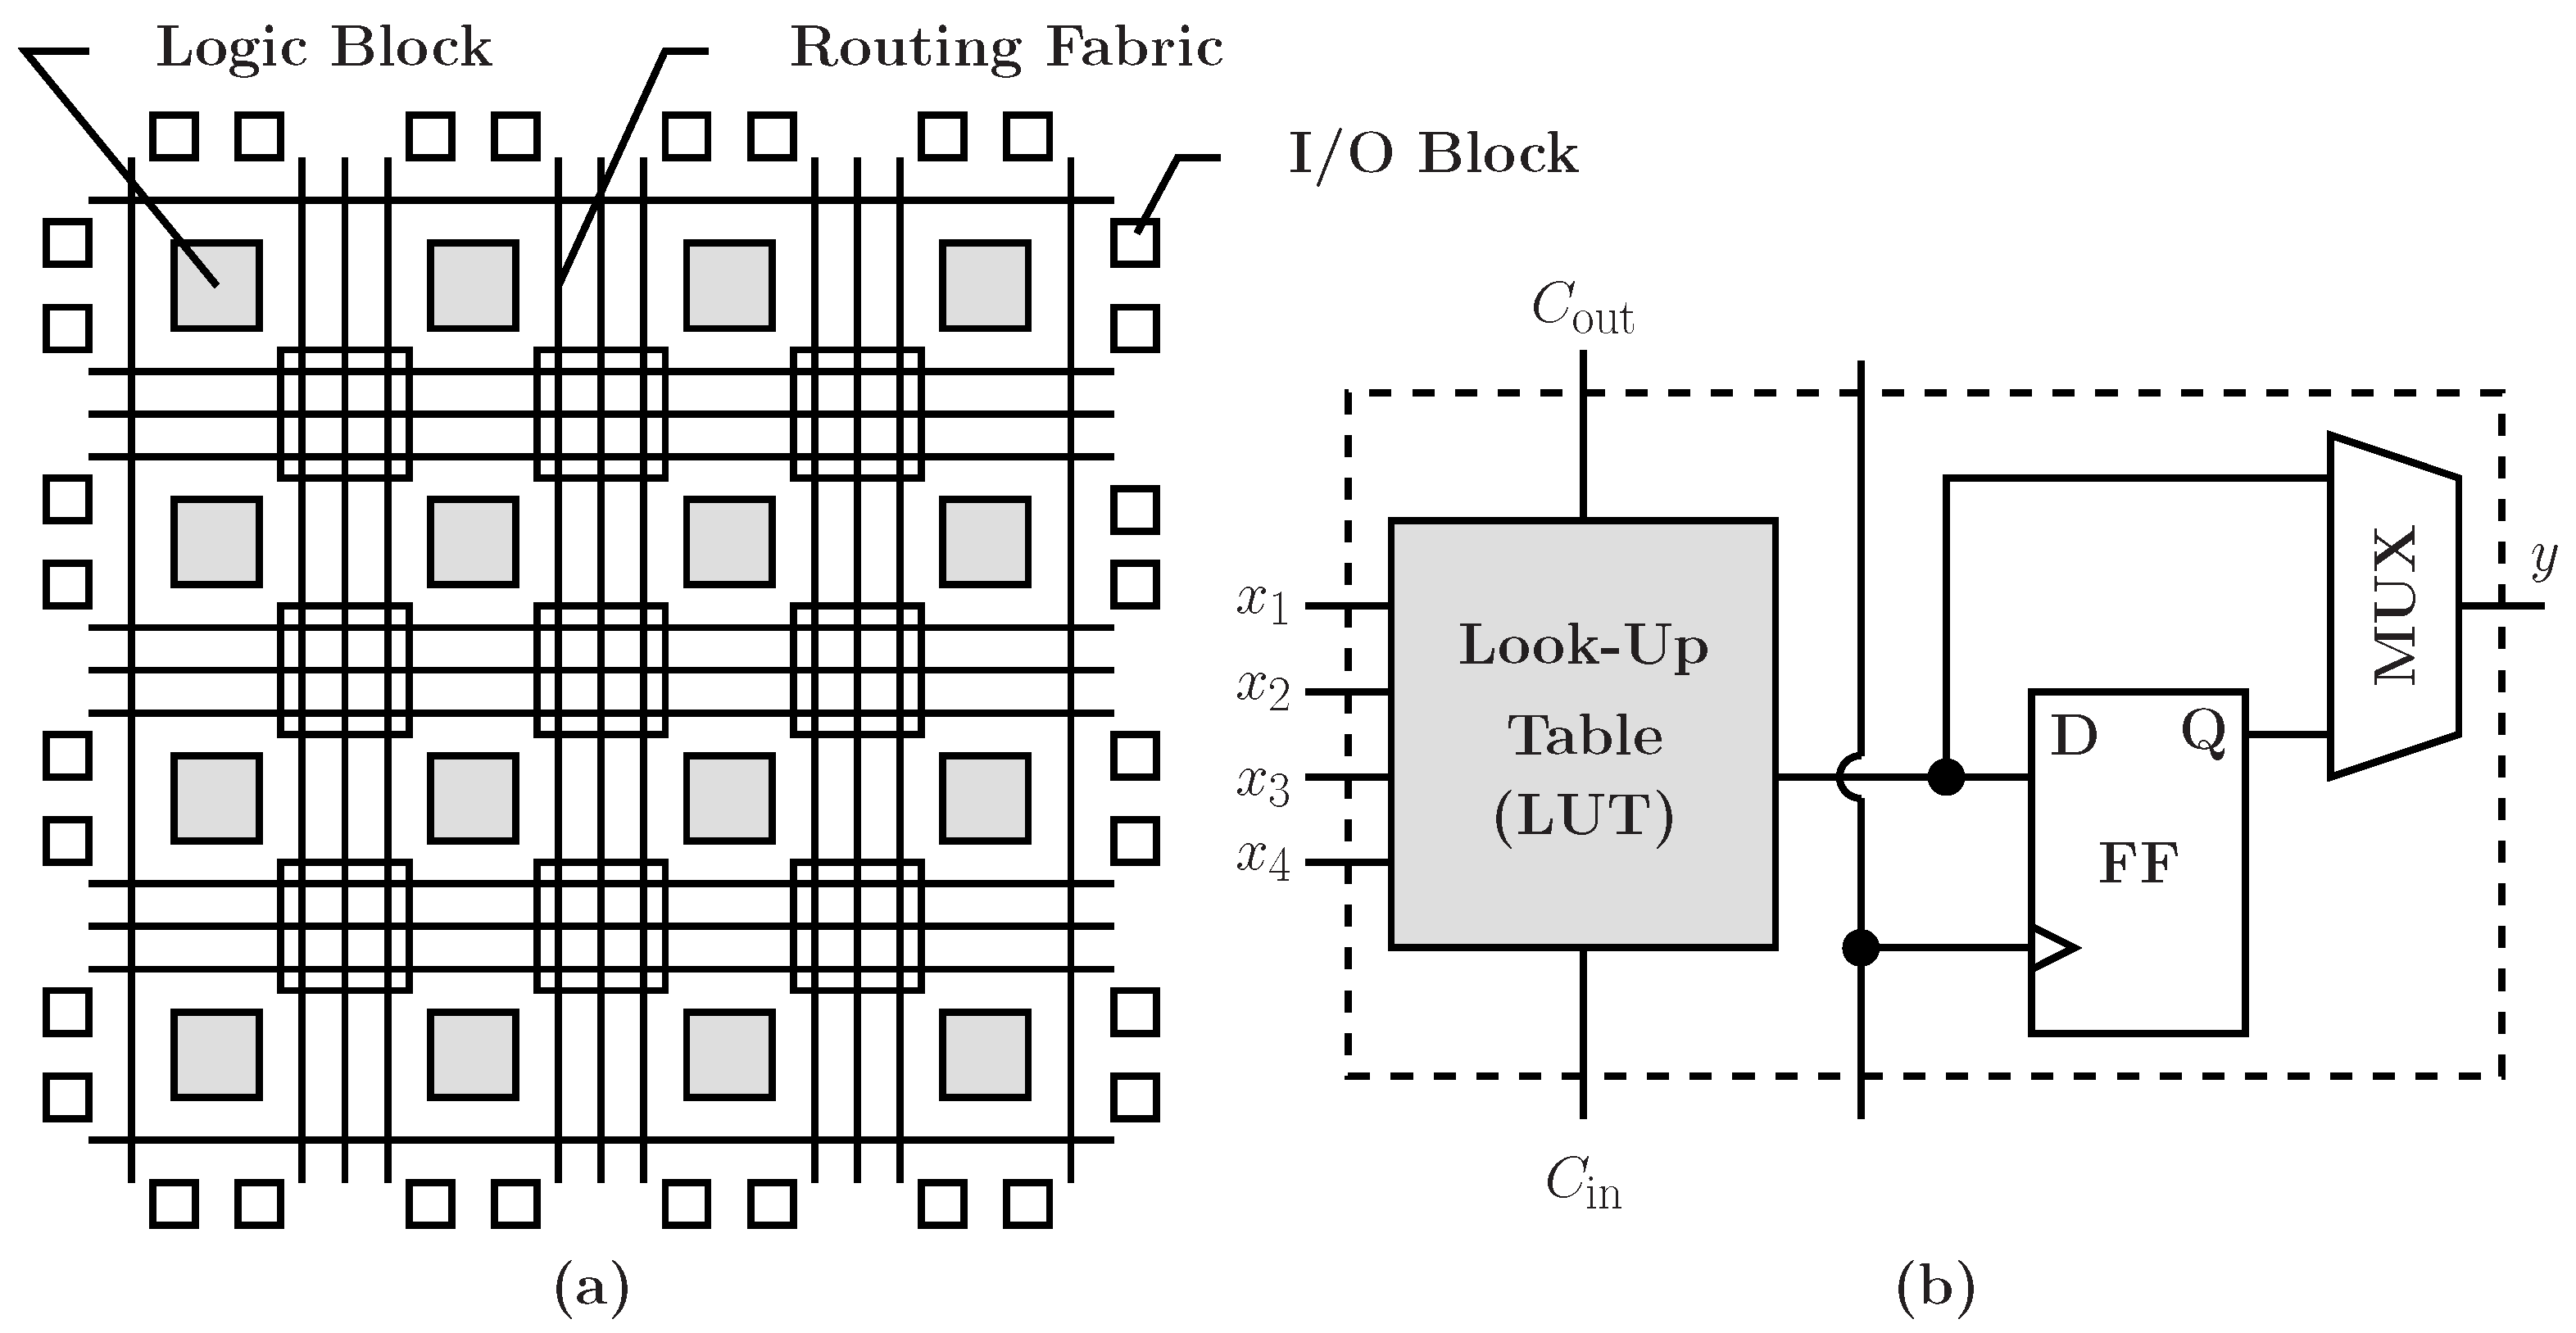
\includegraphics[]{fpga1}
	\caption{Schema FPGA}
\end{figure}

\section{Scrivere e compilare System Verilog}

Creiamo un multiplexer da due bit con System Verilog, compiliamo e visualizziamo con \textbf{GTKWave}

\includecode[verilog]{./verilog/2x1mux/mux.sv}{mux.sv}
\includecode[verilog]{./verilog/2x1mux/test_mux.sv}{test\_mux.sv}

Per compilare, eseguiamo da terminale 
\begin{lstlisting}[style={bash}]
iverilog -g2005-sv nome_sorgente.sv -o nome_eseguibile
\end{lstlisting}

Quindi, per compilare entrambi i file e caricarli in GTKWave:
\begin{lstlisting}[style={bash}]
iverilog -g2005-sv test_mux.sv mux.sv -o test_mux
# Eseguiamo la simulazione
./test_mux
# Viene creato il file provamux.vcd, carichiamolo in GTKWave
gtkwave provamux.vcd &
\end{lstlisting}

\includecode[verilog]{./verilog/2x1mux/mux4.sv}{Multiplexer da 4 vie ad 1 bit}

\includecode[verilog]{./verilog/2x1mux/muxbool.sv}{Multiplexer di variabili booleane}

\clearpage

\section{Esercizi}
\subsection{Automa che riconosce "abba"}

Realizziamo un automa di Mealy che riconosce le stringhe \textit{"abba"} da un insieme $ \{a,b,c\} $. La rete sequenziale dell'automa si realizzerà con i componenti visti in figura ~\ref{fig:mealyautomata1.tex}. Consideriamo la rappresentazione binaria dell'alfabeto con $ a = 00, b = 01, c = 11 $. Per gli stati usiamo la codifica $ S_1 = 00, S_2 = 01, S_3 = 11, S_4 = 10 $

\begin{figure}[H]
	\centering
	\caption{Automa di Mealy che riconosce "abba"}
	\begin{tikzpicture}[->,>=stealth',shorten >=1pt,auto,node distance=3.5cm]
	
	\node[state,accepting] 	(A)                    {$S_1$};
	\node[state]         	(B) [above right of=A] 	   {$S_2$};
	\node[state]         	(C) [below right of=B] 	   {$S_3$};
	\node[state]         	(D) [below right of=A] 	   {$S_4$};
	
	\path 	(A)		edge [bend left]  	node {$a/0$} 		(B)
	edge [loop left] 	node {$b,c/0$} 		(A)
	(B) 	edge [loop above] 	node {$a/0$} 		(B)
	edge [bend left] 	node {$c/0$} 		(A)
	edge [bend left]  	node {$b/0$} 		(C)
	(C)		edge [bend left]  	node {$c/0$} 		(A)
	edge [bend left]  	node {$a/0$} 		(B)
	edge [bend left]  	node {$b/0$} 		(D)
	(D)		edge [bend left]  	node {$b,c/0$} 		(A);
	\end{tikzpicture}
\end{figure}

\begin{table}[H]
	\centering
	\caption{Tabella di verità dell'output della rete sequenziale dell'automa "abba" ($ \omega $)}
	\label{tab:mealyomega2}
	\begin{tabular}{l|llll|l|}
		\cline{2-6}
		& $s_1$ & $s_2$ & $x_1$ & $x_2$ & z \\ \cline{2-6} 
		Stato $S_1$ & 0     & 0     & -     & -     & 0 \\
		Stato $S_2$ & 0     & 1     & -     & -     & 0 \\
		Stato $S_3$ & 1     & 1     & -     & -     & 0 \\
		Stato $S_4$ & 1     & 0     & 0     & 0     & 1 \\
		& 1     & 0     & 0     & 1     & 0 \\
		& 1     & 0     & 1     & 1     & 0 \\ \cline{2-6} 
	\end{tabular}
\end{table}

\begin{table}[H]
	\centering
	\caption{Tabella di verità del cambio di stato dell'automa per riconoscere "abba" ($\sigma$)}
	\label{tab:mealysigma2}
	\begin{tabular}{l|llll|ll|}
		\cline{2-7}
		& $s_1$ & $s_2$ & $x_1$ & $x_2$ & $s_1'$ & $s_2'$ \\ \cline{2-7} 
		Stato $S_1$ & 0     & 0     & 0     & 0     & 0      & 1      \\
		& 0     & 0     & 0     & 1     & 0      & 0      \\
		& 0     & 0     & 1     & 1     & 0      & 0      \\ \cline{2-7} 
		Stato $S_2$ & 0     & 1     & 0     & 0     & 0      & 1      \\
		& 0     & 1     & 0     & 1     & 1      & 1      \\
		& 0     & 1     & 1     & 1     & 0      & 0      \\ \cline{2-7} 
		Stato $S_3$ & 1     & 1     & 0     & 0     & 0      & 1      \\
		& 1     & 1     & 0     & 1     & 1      & 0      \\
		& 1     & 1     & 1     & 1     & 0      & 0      \\ \cline{2-7} 
		Stato $S_4$ & 1     & 0     & 0     & 0     & 0      & 0      \\
		& 1     & 0     & 0     & 1     & 0      & 0      \\
		& 1     & 0     & 1     & 1     & 0      & 0      \\ \cline{2-7} 
	\end{tabular}
\end{table}

% TODO mappa di karnaugh di s1 e s2

Avremo che la formula booleana sarà per il primo e secondo bit di stato:
\[ s_1' = \overbar{s_1}s_2\overbar{x_1}x_2 + s_1s_2\overbar{x_1}x_2 = s_2\overbar{x_1}x_2 \]. 
\[ s_2' = \overbar{s_1s_2}+ \overbar{s_1}s_2\overbar{x_1} + s_2\overbar{x_2}\]

La formula per l'uscita sarà $ z = s_1\overbar{s_2x_1x_2} $. Ci rimane da definire il registro da 2 bit per definire tutta la rete sequenziale. Abbiamo supposto che la rete sequenziale funzioni ricevendo un segnale di clock ad intervalli regolari.
La rete di output $ \omega $ è definita utilizzando soltanto AND ed impiegherà $ \Delta t $ per eseguire l'operazione. La funzione di cambio di stato $ \sigma $ è definita invece con 1 AND e 1 OR ed impiegherà $ 2\Delta t $ per l'operazione.
Il ciclo di clock dev'essere almeno $ \tau = \delta + \max\{t_{\sigma}, t_{\omega}\} $ dove $ \delta $ è la durata del segnale HIGH nel clock.

Abbiamo 3 moduli. Uno per il registro, uno per il modulo $ \omega $ e uno per il modulo $ \sigma $. Scriviamolo in Verilog.

\paragraph{Note}

La sintassi \verb|[a:b]| denota un array indicizzato dal numero \verb|a| al numero \verb|b|. Utilizziamo gli array per rappresentare valori a più bit. In questo caso, il registro è generalizzato per un parametro \verb|N| e può ad esempio essere inizializzato con \verb|registro #(4) nome(...) | dove 4 è il parametro \verb|N| e corrisponde al numero di bit del registro.

La negazione con \verb|!| nega un singolo valore, mentre la notazione \verb|~| viene detta negazione \textit{bit wise} e nega tutti i valori di una sequenza di bit.

Normalmente, in un blocco \verb|assign| assegno un valore ad una variabile booleana istantaneamente. Posso invece aggiungere un delay inserendo \verb|#x| di fronte all'identificatore della variabile, dove \verb|x| è un numero. Ad esempio:
\begin{lstlisting}[style={verilog}]
assign 
	#1 z = (ic == 0 ? x : y)
\end{lstlisting}

\includecode[verilog]{./verilog/abba/Registro/reg.v}{Registro a N bit}
\includecode[verilog]{./verilog/abba/Mealy/sigma.v}{Modulo di $ \sigma $ o funzione di cambio di stato}
\includecode[verilog]{./verilog/abba/Mealy/omega.v}{Modulo di $ \omega $}
\includecode[verilog]{./verilog/abba/Mealy/m1.v}{Modulo della rete sequenziale}
\includecode[verilog]{./verilog/abba/Mealy/test-m1.v}{Modulo di test della rete sequenziale}

\clearpage

\subsection{Automa di Moore per riconoscere "abba"}
Vediamo adesso un automa di Moore per riconoscere la stringa \textit{"abba"} nell'alfabeto $ \{a,b,c\} $. La differenza sta nel fatto che i singoli nodi non hanno accesso all'input $ x $.

\begin{figure}
	\centering
	\caption{Automa di Moore che riconosce "abba"}
	\begin{tikzpicture}[->,>=stealth',shorten >=1pt,auto,node distance=3.5cm]
	
	\node[state,initial] 	(A)                    {$\dfrac{S_1}{0}$};
	\node[state]         	(B) [right of=A] 	   {$\dfrac{S_2}{0}$};
	\node[state]         	(C) [below of=A] 	   {$\dfrac{S_3}{0}$};
	\node[state]         	(D) [below of=B] 	   {$\dfrac{S_4}{0}$};
	\node[state,accepting]  (E) [above right of=D] 	   {$\dfrac{S_4}{0}$};
	
	\path 	(A)		edge [bend left=60]  				node {$a$} 		(B)
					edge [loop above] 					node {$b,c$} 	(A)
			(B) 	edge [loop above] 					node {$a$} 		(B)
					edge [] 							node {$c$} 		(A)
					edge [bend left=20]  				node {$b$} 		(C)
			(C)		edge []  							node {$c$} 		(A)
					edge [bend left=20]  				node {$a$} 		(B)
					edge []  							node {$b$} 		(D)
			(D)		edge [bend left=90,looseness=2]		node {$b,c$} 	(A)
					edge []								node {$a$}		(E)
			(E)		edge [bend right=90,looseness=1.8]  	node {$b,c$} 	(A)
					edge []	node {$a$}		(B);
	\end{tikzpicture}
\end{figure}

\includecode[verilog]{./verilog/abba/Moore/mo-sigma.v}{Modulo di $ \sigma $ o funzione di cambio di stato (Moore)}
\includecode[verilog]{./verilog/abba/Moore/mo-omega.v}{Modulo di $ \omega $ (Moore)}
\includecode[verilog]{./verilog/abba/Moore/moore.v}{Modulo della rete sequenziale (Moore)}
\includecode[verilog]{./verilog/abba/Moore/test-m1.v}{Modulo di test della rete sequenziale (Moore)}
\includecode[makefile]{./verilog/abba/Moore/makefile}{Makefile (Moore)}

\FloatBarrier

\subsection{Mealy con Delay $ \equiv $ Moore}

\includecode[verilog]{./verilog/abba/MealyConDelay/reg-delay.v}{Registro a N bit con delay}
\includecode[verilog]{./verilog/abba/MealyConDelay/sigma-delay.v}{Modulo di $ \sigma $ o funzione di cambio di stato (Mealy con Delay)}
\includecode[verilog]{./verilog/abba/MealyConDelay/omega-delay.v}{Modulo di $ \omega $ (Mealy con Delay)}
\includecode[verilog]{./verilog/abba/MealyConDelay/m1-delay.v}{Modulo della rete sequenziale (Mealy con Delay)}
\includecode[verilog]{./verilog/abba/MealyConDelay/test-m1-delay.v}{Modulo di test della rete sequenziale (Mealy con Delay)}
\includecode[makefile]{./verilog/abba/MealyConDelay/makefile}{Makefile (Mealy con Delay)}

Per sincronizzare il modulo della rete sequenziale dell'automa di Mealy mettiamo un registro di fra l'input \verb|x| e le reti sequenziali \verb|sigma| e \verb|omega|
\chapter{Memorie e Parallelismo}

\section{Memorie}
Un componente fondamentale di un processore è la \textbf{memoria}. Si implementa utilizzando dei registri da $ n $ bit (dette parole). Vogliamo realizzare una memoria il cui accesso sia simile ad un array nel linguaggio C. Ovvero vogliamo avere un vettore di registri a cui possiamo accedere con un offset intero. Data una memoria $ A $ si accederà alla parola $ k-esima $ tramite $ A[k] $. Per implementare tale selezione si può utilizzare un multiplexer che riceve in input le uscite dei singoli registri. I singoli registri ricevono tutti un segnale di clock in input, e permettono la scrittura attraverso un demultiplexer (decoder) che dato un indirizzo invia un 1 all'enable del registro selezionato. Si può mettere in AND il segnale enable del decoder insieme ad un input enable generale.

L'implementazione reale delle memorie (in particolare memorie flash), avviene ponendo delle linee dette "di parola" (orizzontali) e linee dette "bit line" (verticali) in una matrice.
All'incrocio delle linee vi è un condensatore. Il condensatore mantiene una carica per un breve periodo di tempo. Ho modo di controllare se nel condensatore alla posizione $ xy $ era "ricordato" un valore 1, mandando della corrente lungo la "linea di parola" $ x $. Se il condensatore era carico esso si scarica lungo la linea "bit line" $ y $. Inviando della corrente sulla linea di parola $ x $ leggeremo quindi dalle bit line (in alcuni casi indicate come source lines in output) la parola $ x $.
Prima di un condensatore, si inserisce un transistor nella giunzione fra WL e BL. Utilizzando un condensatore, nelle RAM dinamiche (Dynamic Random Access Memory) possono insorgere problemi dovuti ai tempi di carica e scarica del condensatore. Una volta letto un valore su una Bit Line, il condensatore si scarica e "perde" il valore precedentemente "ricordato".

\centerfig{0.65}{flashmem}{Memoria Flash}

Per selezionare la Word Line utilizziamo sempre un demultiplexer (decoder) che riceve un indirizzo. Nelle ram DDR comuni sono presenti spesso 8 o 9 chip. Ad esempio, su uno stick di ram DDR3 da 1GB (1 Giga Byte) sono presenti 8 memorie da 1Gb (1 Giga Bit), e generalmente anche una nona memoria che ricorda la "parità" per il controllo degli errori. Le RAM dinamiche perdono il loro contenuto se non sono alimentate. Visto il comportamento dei condensatori (la loro carica si perde lentamente) le DRAM hanno bisogno di un \textbf{refresh} periodico. Le DRAM sono molto economiche (1 transistor per 1 bit) ma possono risultare più lente rispetto alle alternative SRAM. Le memorie SRAM (Static RAM) sono meno economiche ma più rapide rispetto alle DRAM. Utilizzano flip-flop invece dei condensatori e per ogni bit utilizzano 6 transistor. Le memorie all'interno del processore (calcolatore) sono memorie statiche (realizzate con flip-flop) molto rapide. Un meccanismo sia a livello hardware che a livello di S.O. permette la suddivisione dei dati processati fra vari livelli di cache, dalla memoria statica del processore alla più capiente ma lenta DRAM.

\centerfig{0.35}{dramcell}{Schema di una cella di una memoria DRAM}

\begin{defn}
	\textbf{RAM, ROM, PROM e EEPROM:}
	L'acronimo RAM (Random Access Memory) indica in generale delle memorie sulle quali possiamo leggere e scrivere. Le memorie ROM sono memorie a sola lettura (Read Only Memory). Le memorie ROM non hanno condensatori nelle giunzioni della matrice, ma a momento di produzione vengono "incisi" dei collegamenti o isolamenti nelle giunzioni fra Word Line e Bit Line.
	Le memorie \textbf{PROM} utilizzano dei fusibili nelle giunzioni fra WL e BL per permettere agli acquirenti di scrivere nella memoria una volta sola. Di fabbrica tutti i bit di una PROM sono impostati a 1. Bruciando i fusibili nelle giunzioni si interrompono i collegamenti realizzando una vera e propria scrittura permanente. 
	
	\centerfig{0.65}{prom}{Esempio di memoria PROM}
	
	Un altro tipo di memorie sono le \textbf{EEPROM} (Electrically Erasable ROM). Utilizzano dei transistor particolari che possono essere "reimpostati" permettendo di cancellare e riscrivere la memoria con una corrente maggiore.
	
	Nella seconda parte del corso vedremo dettagliatamente Assembly ARM. Le istruzioni Assembly eseguono delle operazioni sui registri interni alla CPU.
	Un esempio di istruzione banale è la somma di numeri fra registri. \verb|ADD R1 R2 R3|. Nell'Assembly ARM la lettura avviene da destra a sinistra, ed il risultato viene memorizzato nel registro più a sinistra, in questo caso \verb|R1|.	
\end{defn}



\paragraph{Memorie Multi Porta e Tempi di Accesso}
Le memorie multiporta permettono la lettura parallela di due o più registri. Invece di un singolo multiplexer per leggere un registro, alle uscite dei registri è collegato un altro multiplexer che ricevendo un indirizzo diverso dal primo multiplexer, permette di leggere un altro valore dalla memoria, abilitando alla lettura parallela di due registri contemporaneamente. È fondamentale avere una memoria con almeno due porte per eseguire istruzioni su due registri alla volta. Indichiamo i tempi di accesso alla memoria con $ T_a $. Ad oggi siamo in un range di tempi inferiori ad un nanosecondo per i tempi di accesso ai flip-flop (poche decine di picosecondi), sull'ordine dei nanosecondi per le SRAM (cache) e sull'ordine dei microsecondi per le DRAM.


\centerfig{0.75}{DRAM512}{Modulo RAM Corsair DDR2-533}

\paragraph{Blocco memoria}
Introduciamo un blocco per la memoria da utilizzare nei diagrammi dei circuiti.
La memoria riceve in input un dato $ x $ da scrivere nell'indirizzo indicato dall'input di controllo \textbf{Address}. Se il segnale \textbf{enable} è HIGH allora avviene la scrittura di $ x $ all'interno dell'indirizzo puntato. Altrimenti, se \textbf{enable} è LOW avviene la lettura. Assumiamo che l'uscita sia stabile per il ciclo di clock
\diagram{memoryblock.tex}{Blocco Memoria}

\paragraph{LUT (Lookup Table)}
Una rete combinatoria che riceve $ n $ bit in input può essere implementata con una memoria ROM. Data una tabella di verità di una rete combinatoria, si può portare la tabella di verità in forma vettoriale per creare una LUT.
Una LUT o \textbf{Lookup Table} è in generale un array che rimpiazza una computazione, possibilmente complessa, con un operazione di accesso, nel caso delle reti combinatorie con una memoria ROM.
I bit in input della tabella di verità vengono portati a bit rappresentanti l'indirizzo di accesso della memoria, e i risultati della tabella di verità saranno memorizzati in un vettore di $ 2^n $ elementi (se la tabella di verità ha un solo output). 
Per quanto alcune reti combinatorie possono risultare più complesse a livello di circuito se implementate con una LUT, un vantaggio non banale delle Lookup Tables è che possono essere riprogrammate se viene utilizzata una memoria EEPROM. Ciò svolge un ruolo fondamentale negli FPGA. Le LUT possono essere utilizzate in parallelo.

\begin{exmp}
	\textbf{Rete Sequenziale di un contatore}
	Se volessimo realizzare un contatore, con le sole operazioni di incremento e decremento con un ASF, dovremmo avere un numero di stati pari alla capacità massima del contatore.
	Per realizzare un contatore sono necessari un registro da $ n $ bit, (prendiamo ad esempio 8 bit) ed una ALU che fa due sole operazioni (+1 e -1), quindi con un solo bit di controllo. Scegliamo se aumentare o decrementare il contatore impostando il bit di controllo della ALU, e scegliamo se scrivere nel prossimo ciclo di clock impostando ad HIGH il bit Enable (Event) del registro. Essendo una rete sequenziale, la funzione $ \sigma $ è implementata dalla ALU, e la funzione $ \omega $ è semplicemente l'identità. È una rete di Moore poiché la funzione identità non dipende dagli ingressi (Inc/Dec ed Event).
	
	\diagram{counter.tex}{Rete sequenziale di un contatore}
\end{exmp}


\begin{exmp}
	\textbf{Semplice Calcolatrice}
	Vogliamo realizzare una calcolatrice molto semplice da 32 bit per eseguire addizione, sottrazione, moltiplicazione e divisione. La calcolatrice riceverà in input due numeri $ A,B $ e restituirà in output il risultato, che potrà essere re-inserito nei due registri contenenti $ A $ e $ B $. Essa è una rete sequenziale che possiamo inserire in un componente che avrà in input i due numeri $ A,B $, la selezione dei due multiplexer per gli input, segnali di enable per la scrittura nel registro $ A $ e nel registro $ B $ e due bit di controllo per selezionare l'operazione. In output avrà il numero in uscita e 4 bit di flag (Overflow, Carry, Negative e Zero). Definiamo questa parte del calcolatore "parte operativa". Abbiamo bisogno anche di una "parte di controllo" che dati due input si occuperà di controllare le entrate di controllo della parte operativa della calcolatrice.
	
	\diagram{calculator.tex}{Semplice Calcolatore (Omesso clock per semplicità del disegno, è presente)}
\end{exmp}


\begin{defn}
	\textbf{if-then-else:}
	Supponiamo di voler realizzare un importante costrutto per la programmazione (\textit{if-then-else}) utilizzando solo componenti standard. Abbiamo due reti combinatorie $ f,g $, una parola memorizzata in un registro $ A $ e un registro $ B $ in cui sarà memorizzato il risultato. Vogliamo costruire una rete per evaluare l'espressione:
	
	\begin{Verbatim}
	if(expr) then
		g(A) -> B
	else
		f(A) -> B
	\end{Verbatim}
	
	\diagram{ifthenelse.tex}{Rete che implementa if-then-else}
\end{defn}

\begin{defn}
	\textbf{while:}
	Se volessimo invece implementare un ciclo while della forma:
	\begin{Verbatim}
	while(expr) do
	f(A) -> A
	\end{Verbatim}
	Possiamo realizzarlo con la seguente rete:
	
	\diagram{while.tex}{Rete che implementa while}
	
	In maniera simile è possibile realizzare anche un costrutto switch-case.
	Icarus Verilog, per trasformare programmi Verilog di moduli behavioural in netlist di componenti di reti logiche utilizza meccanismi simili.
\end{defn}

\begin{exrc}
	\textbf{Confronto maggiore}
	
	Vediamo ora diversi metodi per realizzare una rete combinatoria che controlla se un numero è maggiore di un altro, utile per realizzare operazioni condizionali.
	
	\includecode[verilog]{./verilog/confrontomaggiore/maggioreb.v}{Esercizio di confronto maggiore in Verilog (approccio algoritmico)}
	
	\FloatBarrier	
\end{exrc}


\subsection{Calcolatrice con registri di memoria}
Realizziamo adesso una calcolatrice con sottrazione e addizione che permette di leggere due numeri in input e fare operazioni utilizzando anche numeri precedentemente memorizzati in degli altri registri. Abbiamo bisogno di risorse di calcolo (una ALU) e registri o memorie. Abbiamo bisogno di una memoria multiporta particolare per realizzare correttamente il circuito. Questa memoria accetta 3 indirizzi, i primi due sono per la lettura (ha due parole in output) e il terzo indirizzo è per la scrittura. È una rete sequenziale, per questo motivo abbiamo bisogno di un meccanismo per evitare i problemi di temporizzazione. Essendo una rete sequenziale il tempo di esecuzione sarà $ \tau = \delta + \max\{t_\sigma, t_\omega\} $. Dovremmo prendere un tempo del ciclo di clock $ \tau = \delta + \max \left\{\begin{matrix}
t_\text{MUX} + t_\text{ALU}, \\
t_\text{ALU} + t_\text{MUX}
\end{matrix}\right\} $ dove $ t_\sigma = t_\text{MUX} + t_\text{ALU} $ e $ t_\omega = t_\text{ALU} + t_\text{MUX} $

\diagram{calculatormemory.tex}{Calcolatrice con memoria.}

%TODO codice verilog

\section{Parallelismo}

\begin{defn}
	
	Supponiamo di avere una serie di libri $ L_1, L_2, L_3, L_4 $ da tradurre. Vogliamo ridurre il tempo totale di traduzione di tutti i libri. Se a tradurre un libro impiego un tempo da $ t_0 $ a $ t_1 $, suddividendo la traduzione a metà fra due persone, impiegheremo $ t_{1/2} $ a tradurre il libro. L'obiettivo del parallelismo è ridurre la \textbf{latenza}. Se ho un insieme di libri, la latenza $ L $ di un libro è il tempo necessario per tradurlo (il tempo a cui ho terminato la traduzione, meno il tempo in cui ho iniziato la traduzione). Se ho $ m $ task da completare, il \textbf{tempo di completamento}  $ T_c = m \cdot L$ è il tempo totale necessario a completare tutti i task m. Con il parallelismo vogliamo diminuire il tempo di completamento. Con \textbf{tempo di servizio} intendiamo l'intervallo medio di tempo fra la "consegna" di due risultati successivi. Definiamo anche \textbf{throughput} come il numero di calcoli eseguiti per unità di tempo.
	
	Data una lista di istruzioni $ i_0, i_1, i_2, i_3, \dots $ il nostro processore esegue (in pseudocodice):
	
	\begin{lstlisting}
	while(true) {
	leggi un istruzione (ASM)
	interpreta
	esegui
	}
	\end{lstlisting} 
\end{defn}


\begin{defn}
	\textbf{Tempo ideale:}
	Dato $ n = $ numero di worker (o grado di parallelismo) e $ T_{\text{seq}} = $ il tempo sequenziale, il \textbf{tempo ideale} $ T_{\text{id}}(n) = \dfrac{T_{\text{seq}}}{n}$.
\end{defn}


\begin{defn}
	\textbf{Speedup:}
	Definiamo anche lo \textbf{speedup} come $ \dfrac{T_{\text{seq}}}{T(n)} $, ovvero il miglior tempo sequenziale fratto il tempo parallelo con grado di parallelismo $ n $.
\end{defn}

\begin{defn}
	\textbf{Scalabilità:} $ \text{Scalab}(n) = \dfrac{T(1)}{T(n)} \leq n $
\end{defn}

\begin{defn}
	\textbf{Efficienza:}
	$ \text{Efficienza}(n) = \dfrac{T_{\text{id}}}{T(n))} = \dfrac{T_{\text{seq}}/n}{T(n)} = \dfrac{T_{\text{seq}}}{n \cdot T(n)} \leq 1 $
\end{defn}


\begin{defn}
	\textbf{Parallelismo temporale o Pipelining:} Il processore deve sempre eseguire dei task (istruzioni) sequenzialmente per eseguire un programma, e si può diminuire la latenza dei singoli task per ridurre il tempo di esecuzione del programma.
	
	\centerfig{0.75}{pipelining}{Diagramma temporale del pipelining di una CPU.}
	
	Avremo che $ T_c = $ tempo iniziale di "riempimento" della pipeline + tempo $ ( \propto ( m \cdot $ tempo delle singole istruzioni )) 
	
	In alternativa, il nostro processore può assegnare un "ciclo" ad ogni istruzione
	
	\begin{lstlisting}[frame=single]
	// Per istruzione 0
	while(true) {
	leggi, decodifica, esegui
	}
	\end{lstlisting} 
	\begin{lstlisting}[frame=single]
	// Per istruzione 1
	while(true) {
	leggi, decodifica, esegui
	}
	\end{lstlisting} 
	\begin{lstlisting}[frame=single]
	// Per istruzione 2...
	while(true) {
	leggi, decodifica, esegui
	}
	\end{lstlisting} 
	
	\centerfig{0.75}{pipelining2}{Pipelining con più worker (parallelismo temporale).}
	
	Usando il \textbf{parallelismo temporale}, ad ogni periodo $ L $ otterremo 3 risultati. Ciò riduce il tempo di servizio a $ \frac{1}{3}L $. Le istruzioni dei task sono comunque eseguite sequenzialmente su worker separati.	
\end{defn}



\begin{defn}
	\textbf{Parallelismo spaziale:}
	Nel \textbf{parallelismo spaziale}, suddividiamo le istruzioni di ogni task su worker diversi. Significa che i worker possono eseguire in parallelo le istruzioni di un singolo task. Il parallelismo spaziale serve a diminuire la latenza, il parallelismo temporale serve invece ad aumentare il throughput.
	
\end{defn}

%TODO diagramma memorie parallellismo dei moduli di memoria multiplexer 18 ottobre 11:55, togliere multiplexer per parallelizzare.

%TODO diagramma differenza pipeline - farm - map

\paragraph{Pipeline (stream parallel)}

%TODO diagramma pipeline

Avendo 3 worker ed eseguendo 3 istruzioni a cascata che impiegano rispettivamente $ 2t, 3t, 1t $, se eseguiamo dei task successivamente, le istruzioni dei task successivi avverrano con un delay dovuto alla differenza del tempo di esecuzione. Dopo un numero di istruzioni le istruzioni si sincronizzeranno. Se i worker impiegano rispettivamente dei tempi $ t_1,t_2,t_3 $, il tempo di completamento di $ m $ istruzioni sarà $ T_c = \sum t_i + (m + 1) \cdot \max\{t_1,t_2,t_3\} $. Ciò crea una situazione non ottimale

\[ \begin{aligned}
n = \text{numero di stadi della pipeline} \\
T_s = \max\{T_{Si}\} \\
\max(\text{speedup(n)}) = \text{\# di stadi della pipeline} \\
T_c (n) = \sum_i L_i + n-1 T_s
\end{aligned} \]

\centerfig{0.75}{nopipeline}{Processore senza pipeline (sottoscalare)}
\centerfig{0.75}{fivestagespipeline}{Processore con pipeline a cinque stadi (scalare)}
\centerfig{0.75}{Superscalarpipeline}{Processore con pipeline superscalare}

\paragraph{Map e Farm}

% TODO diagramma map 
Farm è di tipo \textit{stream parallel} mentre map è di tipo \textit{data parallel}. Nel caso del \textbf{Map} (e anche del Farm), se le  istruzioni impiegano un tempo $ t $ che viene precisamente suddiviso in $ t/2 $ allora il problema non sussiste. Se invece vengono suddivise in tempi diversi si creano spazi temporali in cui non è possibile sfruttare tutta la potenza di calcolo. Nella map posso suddividere un dato in arrivo e fare del calcolo in parallelo su di esso (\textit{data parallelism}). Nella farm e nella pipeline i dati in arrivo possono essere passati a diversi worker (verrano schedulati) che eseguono computazioni in parallelo (\textit{stream parallelism}). I dati non possono essere suddivisi nello \textit{stream parallelism} come nel \textit{data parallelism}.

\paragraph{Tempi della Farm}
\[ \begin{aligned}
nw = \text{grado di parallelismo}\\
T_w = \text{ il tempo che 1 worker impiega per calcolare 1 risultato} \\
T_s = \max\left\{T_{\text{sched}}, \dfrac{T_w}{nw}, T_{\text{coll}}\right\}
\end{aligned} \]

\paragraph{Tempi della Map}
\[ \begin{aligned}
T_c = T_\text{split} + \dfrac{m}{nw} T_f + T_\text{merge} \\
T_s = \max\left\{T_\text{split}, T_\text{merge}, \dfrac{m}{nw}t_f\right\}
\end{aligned} \]

\subsection{Processore superscalare}

Scriviamo un loop di esecuzione del processore in maniera più accurata.

\begin{lstlisting}[frame=single]
while(true) {
I = fetch(PC) // PC = program counter
decode(I)
exec(I)
|--> update(PC)
}
\end{lstlisting}

% TODO diagramma program counter modulo di memoria sopra, pipeline sotto e superscalare

% TODO diagramma esempio libro

\paragraph{Composizione nel parallelismo}

Possiamo comporre i diversi metodi di parallelismo. Ad esempio si può realizzare una pipeline che contiene una farm. Prendiamo ad esempio

\[ \begin{aligned}
\text{pipe}(S_1, \text{farm}(S_2), S_3) \\
\text{Un possibile schema dei worker della pipeline è} \\
\to f \to \begin{cases}
\text{(farm)} \\
g \\ g
\end{cases} \to h \\
\text{Calcoliamo i tempi} \\
T_s = \max\left\{T_{S_1}, T_{S_2}, T_{S_3}\right\} \\
T_s = \max\left\{T_f, \max\left\{T_\text{sched}, \dfrac{T_g}{nw}, T_\text{coll}\right\}, T_h \right\} \\
= \max\left\{T_f, T_\text{sched}, \dfrac{T_g}{nw}, T_\text{coll}, T_h \right\}
\end{aligned} \]

% TODO maggiore tabella e normale

\begin{defn}
	\textbf{Bottleneck o Colli di Bottiglia}
	
	Supponiamo di avere due computazioni composte $ f \circ g $. Se $ f $ impiega $ 5t $ e $ g $ impiega $ 2t $, eseguire in successione $ \to f \to g \to $ può causare dei bottleneck (rallentamenti). Se $ f $ è data parallel si può suddividere la sua computazione in parti uguali (ad esempio due) e poi passare il risultato a $ g $. In alternativa si può dividere $ f $ in 5 parti uguali e ad ogni parte calcolare la composizione sequenziale (in una farm) in modo che $ T_s = \max\left\{T_\text{sched}, \dfrac{T_w}{nw}, T_\text{coll}\right\} \approx \dfrac{Tw}{nw} \approx \dfrac{7t}{5} \approx 1$

	% TODO diagramma bottleneck
\end{defn}

\begin{exmp}
	\textbf{Pipeline in Verilog}
	
	Vediamo adesso una pipeline per parallelizzare l'operazione di moltiplicazione per 2 composta due volte.
	
	
	\includecode[verilog]{./verilog/2xpipeline/singlestage/per2.v}{Modulo moltiplicazione per 2}
	\includecode[verilog]{./verilog/2xpipeline/singlestage/per4.v}{Modulo moltiplicazione per 4}
	\includecode[verilog]{./verilog/2xpipeline/singlestage/test.v}{Programma di test}
	
	\includecode[verilog]{./verilog/2xpipeline/twostages/per2.v}{Modulo moltiplicazione per 2 (pipelined)}
	\includecode[verilog]{./verilog/2xpipeline/twostages/per4.v}{Modulo moltiplicazione per 4 (pipelined)} 
	\includecode[verilog]{./verilog/2xpipeline/twostages/test.v}{Programma di test (pipelined)}
	
	%TODO immagine gtkwave
\end{exmp}




\backmatter
% bibliography, glossary and index would go here.

\end{document}